\documentclass{standalone}
\usepackage{tikz}
\usetikzlibrary{
  arrows,
  calc,
  decorations.pathmorphing,
  decorations.pathreplacing,
  decorations.markings,
  fadings,
  positioning,
  shapes,
  arrows.meta
}
\pgfdeclareradialshading{glow}{\pgfpoint{0cm}{0cm}}{
  color(0mm)=(white);
  color(5mm)=(white);
  color(9mm)=(black);
  color(10mm)=(black)
}

\begin{tikzfadingfrompicture}[name=glow fading]
  \shade [shading=glow] (0,0) circle (1);
\end{tikzfadingfrompicture}

\ifpdf
% Ensure reproducible output
\pdfinfoomitdate=1
\pdfsuppressptexinfo=-1
\pdftrailerid{}
\fi

\begin{document}

\begin{tikzpicture}[scale=1.3593]
  % f_raman0 = 770.200516(24) MHz
  % f_pa0 = 288711.696(73) GHz
  % offset = 2.194(17) kHz/mW
  % strength = 4.1083(46) MHz GHz/mW
  \node at (-0.1cm - 1pt, 0) {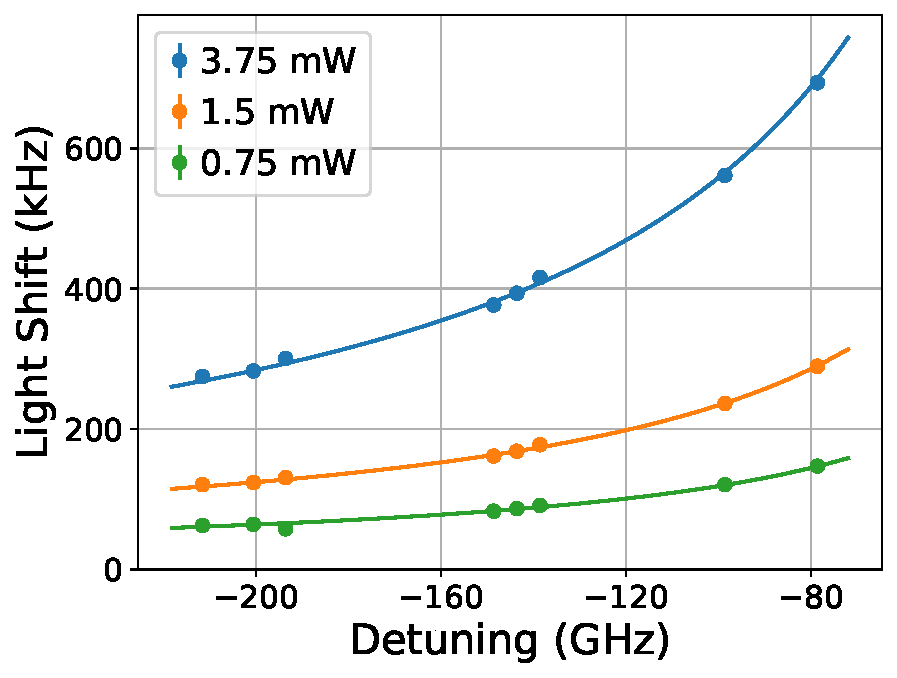
\includegraphics[height=4.7577cm]{imgs/scaling_light_shift.pdf}};
  \node at (-2.0cm - 1pt, 1.5) {\footnotesize (\textbf{a})};
  % offset = -2pi 68.0(53) Hz/mW^-1.29
  % strength = 2pi 25.79(60) kHz GHz/mW^-1.29
  \node at (4.45, 0) {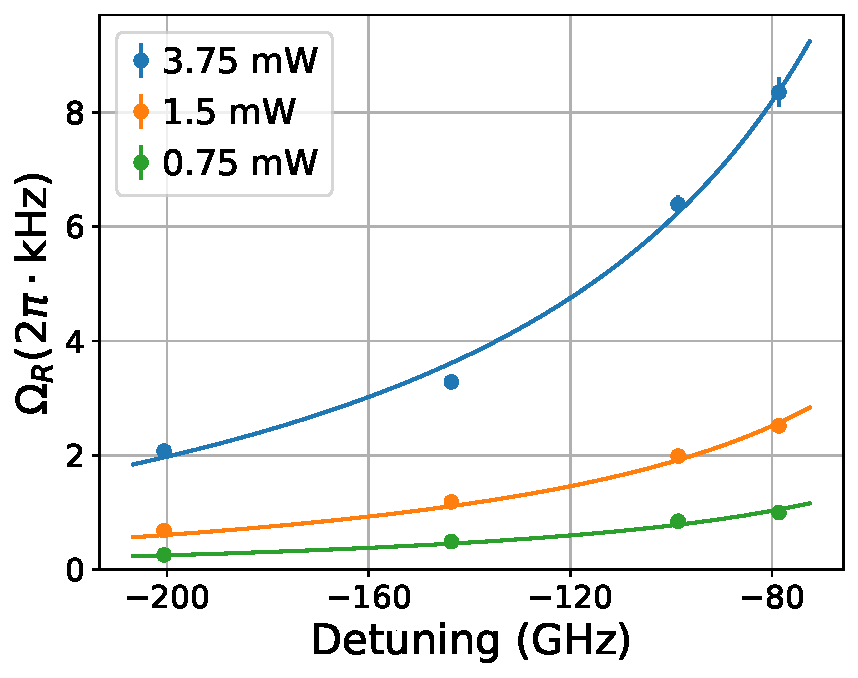
\includegraphics[height=4.7577cm]{imgs/scaling_rabi.pdf}};
  \node at (2.5, 1.5) {\footnotesize (\textbf{b})};
  \node at (8.1cm + 1pt, 0) {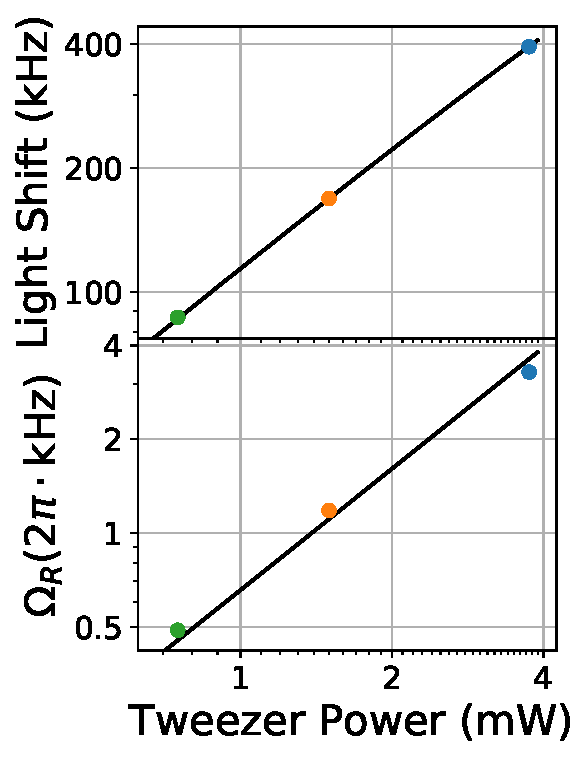
\includegraphics[height=5.0296cm]{imgs/scaling_560.pdf}};
  \node at (7.6cm + 1pt, 1.55) {\footnotesize (\textbf{c})};
\end{tikzpicture}

\end{document}
